\documentclass[a4paper]{article}
\usepackage{geometry}
\usepackage[utf8]{inputenc}
\usepackage[T1]{fontenc}
\usepackage[bookmarks,colorlinks]{hyperref}
\usepackage[french]{babel}
\usepackage{pdflscape}
\usepackage{graphicx}

\title{Rapport d'analyse du projet de Technologies Objets}
\author{Maxime Arthaud \and Korantin Auguste \and Martin Carton}
\date{24 Mai 2013}

\begin{document}
\maketitle

\section{Introduction}
  Ce projet consiste en la création d'une interface utilisateur permettant de
  gérer une scène 3D et à la réalisation d'un moteur de rendu par lancé de
  rayons.

\section{Démarche}
  Nous avons commencé par la liste des choses à faire. Nous avons décidé
  de séparer l'interface graphique du moteur de rendu. L'interface
  graphique permettra de générer un fichier contenant toutes les informations
  de la scène nécessaires à la génération de l'image, qui sera faite par un
  second programme utilisable en ligne de commande, ce fichier sera simple et
  pourra être écrit à la main.

\section{Tâches effectuées}
  Nous avons commencé à réfléchir à l'organisation des classes, à l'interface
  utilisateur et au format de fichier.

  \subsection{Interface utilisateur}
    La figure \ref{fig:gui} présente l'interface graphique telle que nous
    envisageons de la faire.

    Les différents objets (caméra,
    sphères, cubes et plans) peuvent y être ajoutés selon leurs différentes
    propriétés optiques et supprimés. Un résumé des objets créés est affiché, on
    peut directement lancer la génération de l'image, ou enregistrer le fichier.

  \subsection{Format de fichier}
    Le fichier sera un fichier texte où chaque objet sera représenté sur une
    ligne. Chaque ligne sera de la forme
    \verb+Nom(param1=valeur1, param2=valeur2, ..., paramN=valeurN)+
    où \verb+Nom+ est le nom de l'objet à créer (Camera, Sphere, Cube ou
    Plane), et les paramètres et
    valeurs sont les données qui caractérisent l'objet, par exemple le rayon
    et le centre pour la Sphere, ou encore la réflectance.

    Pour simplifier l'écriture manuelle du fichier,
    certains paramètres ont une valeur par défaut, comme l'indice de réfraction.

  \subsection{Moteur de rendu}
    Nous avons décidé de structurer notre programme de la manière suivante:
    tout d'abord, la classe \verb+FileReader+ va se charger de parser le
    fichier décrivant la scène.

    La méthode \verb+computeColor+ sera chargée de donner la couleur d'un rayon
    arrivant sur l'objet (et appellera récursivement cette même méthode pour
    d'autres objets, dans la plupart des cas).
    Une seconde méthode, \verb+distance+, est chargée de donner la distance
    parcourue le long du rayon passé en paramètre pour arriver jusqu'à l'objet.

    Un objet pourra soit être un \verb+Mesh+, composé de plusieurs triangles
    (ce sera le cas d'un \verb+Cube+), soit être un objet possédant toutes les
    caractéristiques optiques nécessaires.

    Il sera donc très facile de générer notre image: il suffira, pour chaque
    rayon commençant par le point de vue de l'observateur et passant par un
    pixel de l'écran, de trouver quel est le premier objet qu'il intersecte
    grâce à la méthode \verb+distance+, et d'utiliser la méthode
    \verb+computeColor+ pour calculer la couleur de ce point de l'objet.

    Les classes \verb+PPMImageWriterSpi+ et 
    \verb+PPMWriter+ permettent de gérer les images au format
    PPM en utilisant les interfaces standards de java, ce qui nous permettra
    de pouvoir exporter aussi bien en PPM qu'en PNG, format supporté par défaut
    par java.

    La figure \ref{fig:uml} présente les relations entre les différentes classes
    que nous envisageons d'utiliser.

\section{Démarche et répartition des tâches} 
  Nous avons décidé de développer l'interface graphique en dernier. Nous 
  comptons faire des tests unitaires pour les classes
  \verb+FileReader+ et \verb+PPMWriter+. Nous ferons des tests d'intégrations
  en maintenant un ensemble de fichiers de scène qui couvrent l'ensemble des
  fonctionnalités du programme.

  Nous avons déjà répartis quelques tâches:
  \begin{itemize}
    \item Maxime: travaillera sur la GUI;
    \item Martin: travaillera sur le parseur et l'enregistrement d'image;
    \item Korantin: rédaction des rapports et comptes rendus, et travail
      sur le moteur de rendu.
  \end{itemize}

  Nous allons tous participer à l'implémentation du moteur de rendu.

  %\subsection{Diagramme de séquence}
    \begin{figure}[p]
      \centerline{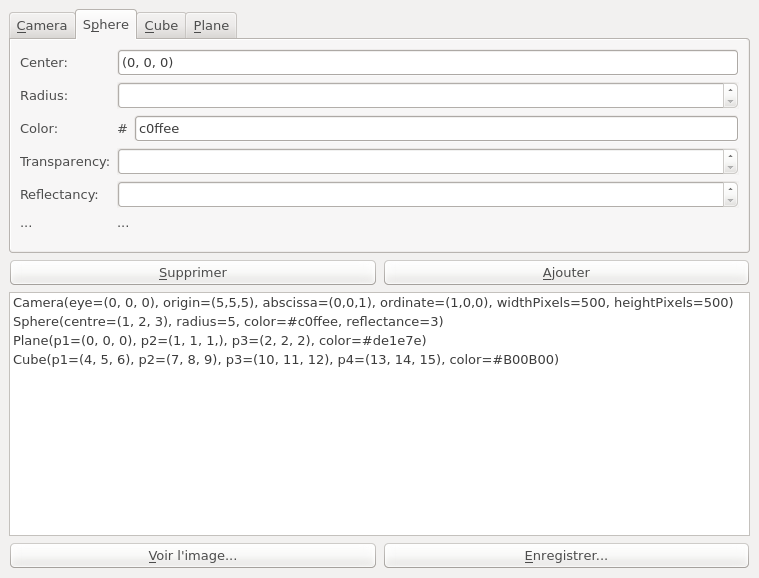
\includegraphics[width=1.2\textwidth]{gui.png}}
    \caption{Interface graphique\label{fig:gui}}
    \end{figure}

    \newgeometry{width=1.3\linewidth}
    \begin{landscape}
      \thispagestyle{empty}
      \begin{figure}[p]
        \makebox[\paperwidth][c]{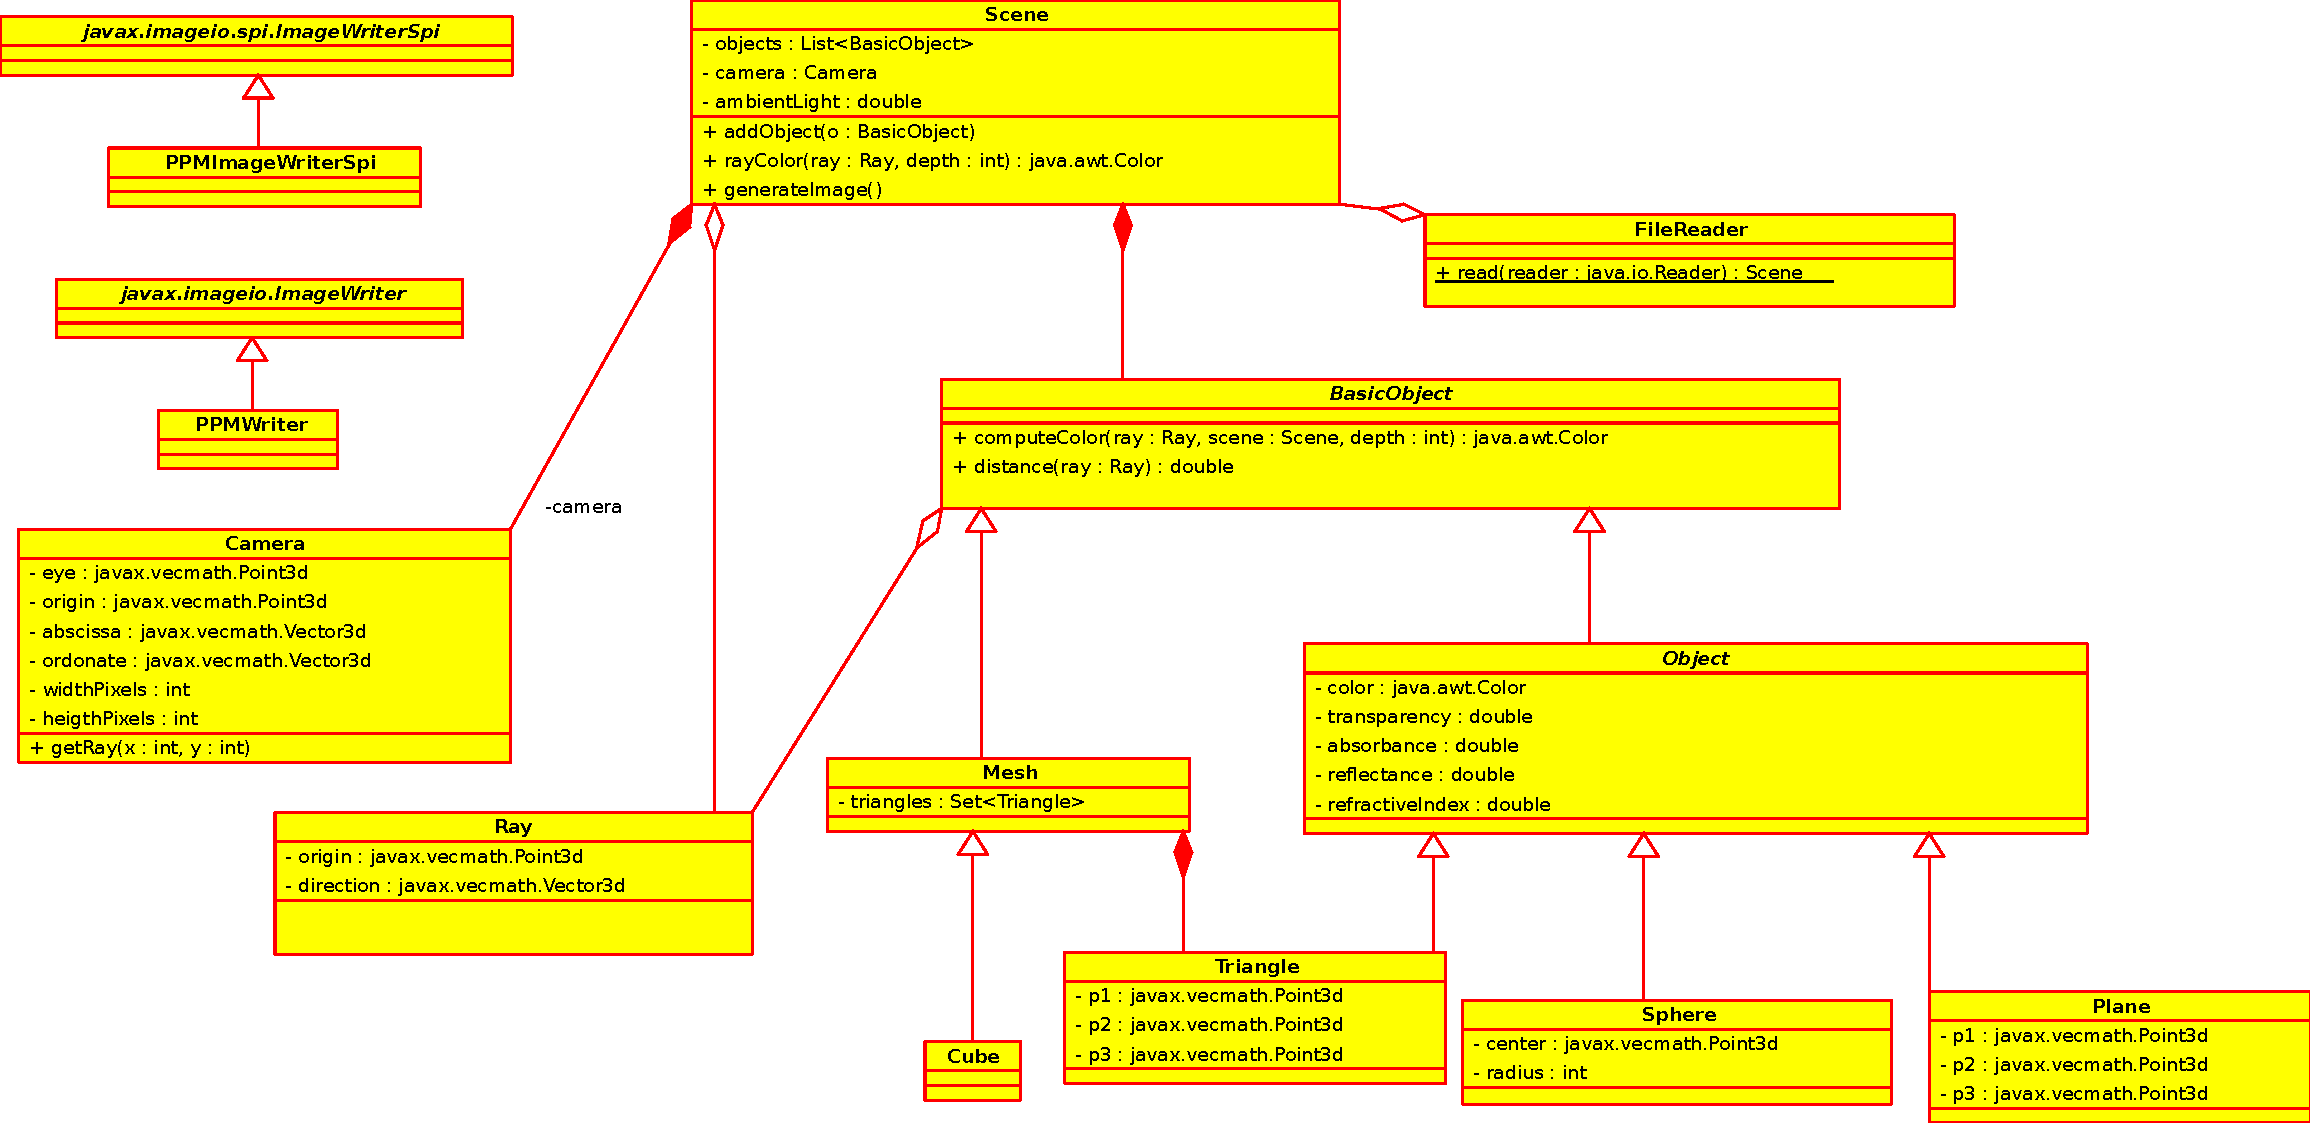
\includegraphics[width=26cm]{uml.pdf}}
        \caption{Diagramme UML\label{fig:uml}}
      \end{figure}
    \end{landscape}
    \restoregeometry
\end{document}

